%==============================================================================
%== template for LATEX poster =================================================
%==============================================================================
%
%--A0 beamer slide-------------------------------------------------------------
\documentclass[final]{beamer}
\usepackage[orientation=portrait,size=a0,
            scale=1.25         % font scale factor
           ]{beamerposter}
           
\geometry{
  hmargin=2.5cm, % little modification of margins
}

%
\usepackage[utf8]{inputenc}
\usepackage{subcaption}


\usepackage{amssymb,amsmath,array}
\usepackage{scalefnt} 
\usepackage{tabularx}
\usepackage{booktabs}
\usepackage[version=4]{mhchem}
\newcommand{\bftab}{\fontseries{b}\selectfont}
\DeclareMathOperator*{\argmin}{\arg \min}
\DeclareMathOperator*{\erro}{\textrm{erro}}
\DeclareMathOperator*{\argmax}{\arg \max}
\usepackage{booktabs}
\usepackage[version=4]{mhchem}
\usepackage{collcell}
\usepackage{scalefnt} 
\usepackage{multirow}
\usepackage{siunitx}
\usepackage{amssymb,array,amsmath}
\sisetup{output-exponent-marker=\ensuremath{\mathrm{e}}}

\usepackage{multirow}
\usepackage{scalefnt} 
\usepackage{graphicx}
\usepackage{color,soul}
\usepackage{setspace}
\usepackage{soul,color}
\usepackage{caption}
% \usepackage[labelformat=simple]{subcaption}
% \renewcommand\thesubfigure{(\alph{subfigure})}
\usepackage{subcaption}
\usepackage{adjustbox}
\usepackage{array}
\usepackage{balance}
\usepackage{colortbl}
\usepackage{tabularx}
\usepackage{booktabs}
\usepackage{hyperref}

\usepackage{pifont}
\newcommand\infe{\textcolor{gray}{\ding{55}}}
\newcommand\supe{\textcolor{gray}{\ding{55}}}
\newcommand\equi{\ding{51}}

\usepackage{pifont}
\usepackage{collcell}
\usepackage{multirow}

\usepackage{algorithm}
\usepackage{algorithmic}
\renewcommand{\vec}{\boldsymbol}
\usepackage{amsthm}



\linespread{1.15}
%
%==The poster style============================================================
\usetheme{sharelatex}

%==Title, date and authors of the poster=======================================
\title
[ESANN, 25 - 27 April 2019, Bruges, Belgium] % Conference
{ % Poster title
Sparse minimal learning machine using\\a diversity measure minimization
}

\author{ % Authors
Madson L. D. Dias$^1$, Lucas S. Sousa$^2$, Ajalmar R. da Rocha Neto$^2$,\\César L. C. Mattos$^1$, João P. P. Gomes$^1$ and T. Kärkkäinen$^3$
}
\institute{1. Federal University of Ceará, Brazil ~
% Department of Computer Science, Brazil\\
% \texttt{\{madson.dias, jpaulo\}@lia.ufc.br}, \texttt{cesarlincoln@dc.ufc.br}
% \vspace{0.5em}
2. Federal Institute of Ceará, Brazil ~
% Department of Teleinformatics, Brazil\\
% \texttt{\{lucas.sousa, ajalmar\}@ppgcc.ifce.edu.br}
3. University of Jyvaskyla, Finland\\
\texttt{madson.dias@lia.ufc.br},
\texttt{lucas.sousa@ppgcc.ifce.edu.br},
\texttt{ajalmar@ifce.edu.br},\\
\texttt{cesarlincoln@dc.ufc.br},
\texttt{jpaulo@lia.ufc.br},
\texttt{tommi.karkkainen@jyu.fi}
}
\date{\today}



\begin{document}
\begin{frame}[t]
%==============================================================================
\begin{multicols}{3}
%==============================================================================
%==The poster content==========================================================
%==============================================================================

\section{Abstract}

\begin{itemize}
\item The minimal learning machine (MLM) training procedure consists in solving a linear system with multiple measurement vectors~(MMV) created between the geometric configurations of points in the input and output spaces. 

\item This paper considers an extension of the focal underdetermined system solver (FOCUSS) for multiple measurement vectors~(MMV) linear systems problems with additive noise, named regularized MMV FOCUSS~(regularized M-FOCUSS), and evaluates it in the task of selecting input reference points (RPs) for regression settings.
\end{itemize}


\section{Minimal Learning Machine~\cite{souza2015}}


\subsection{Definitions}

\begin{itemize}
	\item Data set: $\{(\vec{x}_n, \vec{y}_n)\}_{n=1}^N$
	\item Input points: $\mathcal{X}=\{\vec{x}_n\}_{n=1}^N$ 
	\item Output points: $\mathcal{Y}=\{\vec{y}_n\}_{n=1}^N$ 
    \item Input RPs set: $\mathcal{R} = \{\vec{r}_m\}_{m=1}^M \subseteq \mathcal{X}$
    \item Output RPs set: $\mathcal{T} = \{\vec{t}_k\}_{k=1}^K \subseteq \mathcal{Y}$
    \item[] $\vec{x}_n, \vec{r}_m \in \mathbb{R}^D$ and $\vec{y}_n, \vec{t}_k \in \mathbb{R}^S$
    \item Pairwise distance matrices:\\ $\mathbf{D} \in \mathbb{R}^{N \times M}$ and $\mathbf{\Delta} \in \mathbb{R}^{N \times K}$

    \item Assumption of a linear mapping:
    \begin{equation}
    \mathbf{\Delta} = \mathbf{D} \mathbf{B} + \boldsymbol{\varepsilon}
    \vspace{-1.5em}
    \end{equation}
    \begin{itemize}
    	\item $\mathbf{B} \in \mathbb{R}^{M \times K}$ is the matrix of parameters
    	\item $\boldsymbol{\varepsilon} \in \mathbb{R}^{N \times K}$ denotes the residuals.
    \end{itemize}
\end{itemize}

\subsection{Learning algorithm}
\begin{itemize}
	\item Randomly select a set of reference points from the data
    \item Compute $\mathbf{D}$ and $\mathbf{\Delta}$
    \item Approximate $\mathbf{B}$ by ordinary least squares
    \begin{equation}
    \hat{\mathbf{B}}= (\mathbf{D}^T\mathbf{D})^{-1}\mathbf{D}^T\mathbf{\Delta}. \label{eq: MRLS}
    \end{equation}
\end{itemize}


\subsection{Out-of-sample prediction}

\begin{itemize}
	\item New input point $\vec{x}$
    \item Approximation of the distances $\hat{\vec{\delta}}$  between $\vec{y}$ (the output of point $\vec{x}$) and the output of the RPs:
    \begin{equation}
\hat{\vec{\delta}} = \left[\left \| \vec{x} -  \vec{r}_1 \right \|_2, \cdots, \left \| \vec{x} -  \vec{r}_M \right \|_2 \right] \hat{\mathbf{B}}.
\end{equation}
	\item Output prediction
    \begin{equation}\scalefont{.9}
\hat{\vec{y}} = \arg \min_{\vec{y}} \left\{ \sum_{k=1}^{K}\left( (\vec{y} - \vec{t}_k)^T(\vec{y} - \vec{t}_k) - \hat{\delta}_k^2 \right)^2 \right\}, \label{eq: optimization}
\end{equation}
\end{itemize}


\section{Conventional RPs selection}

\begin{itemize}
    \item The original MLM establishes that the input and output RPs are associated to the same data samples and their selection is made randomly, leaving just the number of points as a user-selected parameter.
    % ~\cite{SouzaJunior2013}
    \item The determination of the reference points, including their quantity, is fundamental to the generalization of the MLM model for classification tasks.
    % ~\cite{dias2018a,maia2018}

    % \item The input RPs are used in the distance approximation step while the output RPs are used in the multilateration step. Therefore, the selection of input and output RPs must be considered as two different tasks.
\end{itemize}


\newpage

\section{Regularized M-FOCUSS ~~~~ minimal learning machine}
\begin{itemize}
    % \item \emph{Regularized M-FOCUSS minimal learning machine}~(RMF-MLM)
    \item \textbf{Idea}: relies on a simultaneous sparse approximation method named regularized M-FOCUSS for the task of identifying which reference points are not relevant to the MLM's performance
    \item This method employs an $\ell_p$-norm-like diversity measure, where $p \in [0,2]$ is a user-defined parameter that indicates the degree of sparsity.
    \item Initially, the RMF-MLM uses all the points as RPs (i.e. $\mathcal{R} = \mathcal{X}$ and $\mathcal{T} = \mathcal{Y}$) to compute the distance matrices $\mathbf{D}$ and $\boldsymbol{\Delta}$. After that, the M-FOCUSS is used to achieve an approximation of $\mathbf{B}$ by finding a local minimum of the following optimization problem
\begin{equation}
\hat{\mathbf{B}} = \arg \min_{\mathbf{B}} \|\mathbf{D}\mathbf{B} - \mathbf{\Delta} \|^2_{\text{F}} + \lambda \sum_{m=1}^{M}  \| \boldsymbol{b}_{m} \|_2^p \label{eq:focuss-cost}
\end{equation}
where $\lambda \geq 0$ is a trade-off parameter balancing estimation quality with diversity measure minimization, and $\boldsymbol{b}_m$ denotes the $m$-th row of $\mathbf{B}$.
\item The regularized M-FOCUSS MLM use the factored-gradient approach of~\cite{rao1999, kreutz-delgado1998} to minimize~(\ref{eq:focuss-cost}). The algorithm iteractively updates $\mathbf{B}$ using the following steps:
\begin{flalign}
\footnotesize \mathbf{W}^{[t+1]} &= \text{diag}\left\{(c_{m}^{[t]})^{1-p/2} \right \} ,~\text{where}~~ c_{m}^{[t]}  =  \left( \sum_{k=1}^{K} \left(b^{[t]}_{km}\right)^2 \right)^{1/2}, \nonumber \\
\footnotesize\mathbf{Q}^{[t+1]} &= \mathbf{D}^{[t+1]T} \left(\mathbf{D}^{[t+1]}\mathbf{D}^{[t+1]T} + \lambda \mathbf{I}\right)^{-1} \boldsymbol{\Delta} ,
\end{flalign}
where $\mathbf{D}^{[t+1]} = \mathbf{D} \mathbf{W}^{[t+1]},$
\begin{flalign}
\footnotesize\mathbf{B}^{[t+1]} &= \mathbf{W}^{[t+1]} \mathbf{Q}^{[t+1]} , \nonumber
\end{flalign}
where $t$ is the the current iterative step and $\mathbf{I} \in \mathbb{R}^{N \times N}$ is an identity matrix. The algorithm is terminated once a convergence criterion has been satisfied, e.g.,
$
    \frac{\| \mathbf{B}^{[t+1]} - \mathbf{B}^{[t]}  \|_{\text{F}}}{\| \mathbf{B}^{[t]}  \|_{\text{F}}} < \tau,
$
where $\tau$ is a the tolerance parameter. In our experiments, was chosen as $0.01$.
\end{itemize}

\section{Experiments}

\begin{itemize}
    \item The performance of RMF-MLM is compared with two variants of the MLM, regarding the selection of input RPs.
    \begin{itemize}
        \item full MLM~(FL-MLM), in which the set of input RPs is equal to the training set (i.e., $\mathcal{R} = \mathcal{X}$).
        \item random MLM (RN-MLM), where we randomly select $M$ input RPs from the training data
    \end{itemize}
    In all of this variants, the whole data outputs are used as RPs (i.e. $\mathcal{T} = \mathcal{Y}$).
\end{itemize}

\subsection{Qualitative analysis}
\begin{itemize}
    \item The toy problem that consists of $200$ points in $\mathbb{R}^2$ regularly spaced in $x$, such that $x_n \in [-3\pi,3\pi]$, $y_n = \frac{\sin{x_n}}{x_n} + \varepsilon$, where~$\varepsilon \sim \mathcal{N}(0, 0.1)$. In this experiment, we use for RN-MLM the number of input reference points found by the RMF-MLM using $p=10^{-5}$ and $\lambda = 10^{-4}$. 
    % Fig.~\ref{fig:decision-surface-1} shows the results of this experiment.
\end{itemize}

\begin{figure}
    \centering
    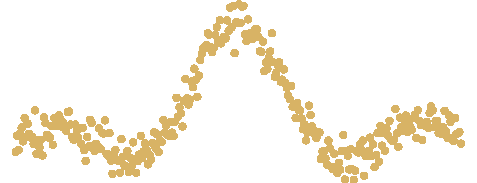
\includegraphics[width=0.28\textwidth]{data.pdf}
    \caption{Artificial data set}
    \label{fig:my_label}
\end{figure}

\newpage 


\begin{figure}
    \centering
    
   \begin{subfigure}[b]{0.28\textwidth}
      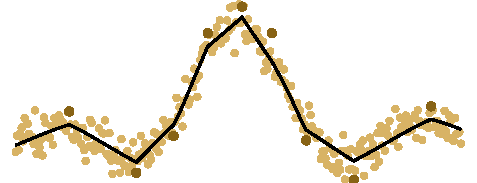
\includegraphics[width=\textwidth]{rmf_mlm.pdf}
      \caption{$|\mathcal{R}|=9$.}\label{fig:results-art_1-dataset}
  \end{subfigure}
  \begin{subfigure}[b]{0.28\textwidth}
      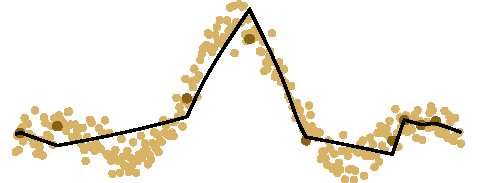
\includegraphics[width=\textwidth]{rn_mlm.pdf}\vspace{-0.1em}
      \caption{$|\mathcal{R}|=9$.}\label{fig:results-art_1-fl}
  \end{subfigure}
  \begin{subfigure}[b]{0.28\textwidth}
      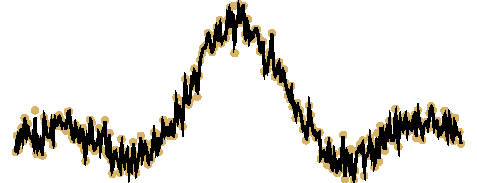
\includegraphics[width=\textwidth]{fl_mlm.pdf}\vspace{-0.1em}
      \caption{$|\mathcal{R}|=200$.}\label{fig:results-art_1-fl}
  \end{subfigure}
    \caption{Model outputs and number of input RPs for~(b)~RMF-MLM, (c)~RN-MLM and~(d)~FL-MLM when applied to ART dataset.}\label{}
\end{figure}



\subsection{Real-world data sets}
\begin{table}[!ht]
\scalefont{0.55}
\caption{Performance comparison -- average values of root mean squared error (RMSE) and number of input reference points (\#IRPs) for the tenfold cross-validation -- with the RMF-MLM, RN-MLM and FL-MLM.}\label{tab:results}
% \vspace{-2em}
\begin{center}
\begin{tabular}{ll r@{${}\pm{}$}l r@{${}\pm{}$}l r@{${}\pm{}$}l r@{${}\pm{}$}l r@{${}\pm{}$}l r@{${}\pm{}$}l}  \toprule
     % &&        &&  \multicolumn{2}{c}{ACC (\%)}     &&                           &&                             \\ \cmidrule{5-6}
\emph{dataset} & \emph{metric}    & \multicolumn{6}{l}{RMF-MLM}   & \multicolumn{2}{l}{RN-MLM} &  \multicolumn{2}{l}{FL-MLM} \\ \cmidrule{3-8}

~& ~    &  \multicolumn{2}{l}{$p = 0.2$} & \multicolumn{2}{l}{$p = 0.4$} & \multicolumn{2}{l}{$p= 1$}   & \multicolumn{2}{l}{~} &  \multicolumn{2}{l}{~} \\ \midrule

\multirow{2}{*}{MTR}  & RMSE    &     23.35 &     7.09 &     23.60 &     6.67 &     23.62 &     6.19 &     25.12 &     5.90 &     30.77 &     8.01 \\ 
                      & \#IRPs  &      9.70 &     0.48 &     11.70 &     0.82 &     26.60 &     1.35 &     27.50 &     8.03 &     84.60 &     0.52 \\ \midrule

\multirow{2}{*}{SRV}  & RMSE    &      0.56 &     0.18 &      0.54 &     0.20 &      0.54 &     0.20 &      0.57 &     0.25 &      0.54 &     0.20 \\ 
                      & \#IRPs  &     38.00 &     1.56 &     63.40 &     2.22 &    139.20 &     1.32 &    114.80 &    21.80 &    150.30 &     0.48 \\ \midrule

\multirow{2}{*}{CPU}  & RMSE    &     43.37 &    22.54 &     47.17 &    31.59 &     45.08 &    24.92 &     53.86 &    39.11 &     45.18 &    19.06 \\ 
                      & \#IRPs  &     12.10 &     0.88 &     21.60 &     6.65 &     67.30 &    14.31 &    137.80 &    48.30 &    188.10 &     0.32 \\ \midrule

\multirow{2}{*}{MGP}  & RMSE    &      2.59 &     0.47 &      2.57 &     0.46 &      2.57 &     0.47 &      2.69 &     0.46 &      2.63 &     0.49 \\ 
                      & \#IRPs  &     49.40 &     2.22 &     89.00 &     2.87 &    238.20 &     3.26 &    194.60 &    70.50 &    352.80 &     0.42 \\ \midrule

\multirow{2}{*}{HSG}  & RMSE    &      2.95 &     0.78 &      2.84 &     0.79 &      2.80 &     0.78 &      2.98 &     0.82 &      2.77 &     0.78 \\ 
                      & \#IRPs  &     85.00 &     3.02 &    160.40 &     5.50 &    380.90 &     2.73 &    406.00 &    57.80 &    455.40 &     0.52 \\ \midrule

\multirow{2}{*}{FFS}  & RMSE    &     60.11 &    44.76 &     56.36 &    46.50 &     57.47 &    46.08 &     48.88 &    47.58 &     55.72 &    47.04 \\ 
                      & \#IRPs  &     35.20 &    15.77 &     69.90 &    29.12 &    230.70 &   102.92 &    247.10 &   117.67 &    465.30 &     0.48 \\ \midrule

\multirow{2}{*}{CCT}  & RMSE    &      6.06 &     0.40 &      5.70 &     0.47 &      5.52 &     0.50 &      5.64 &     0.50 &      5.03 &     0.54 \\ 
                      & \#IRPs  &    173.20 &     4.96 &    307.50 &     3.78 &    722.90 &     5.97 &    816.10 &    76.21 &    927.00 &     0.00 \\ \midrule

\multirow{2}{*}{ABA}  & RMSE    &      2.13 &     0.09 &      2.12 &     0.10 &      2.12 &     0.10 &      2.25 &     0.35 &      2.22 &     0.10 \\ 
                      & \#IRPs  &    220.20 &    19.27 &    334.10 &    17.90 &    752.50 &   28.38 &    688.00 &     20.01 &   3759.30 &     0.48 \\ \bottomrule

% \vspace{-3em}
\end{tabular}
\end{center}
\end{table}




\section{Conclusions}
\begin{itemize}
    \item The proposed approach was called regularized M-FOCUSS minimal learning machine (RMF-MLM). Three strategies of MLM input RPs selection were evaluated. On the basis of our experiments, we can state that RMF-MLM is a promising alternative to select input RPs, providing a competitive model while maintaining its simplicity. 
\end{itemize}


%==============================================================================
%==End of content==============================================================
%==============================================================================

%--References------------------------------------------------------------------

\subsection{References}

\bibliographystyle{ieeetr}
\bibliography{references}


%--End of references-----------------------------------------------------------

\end{multicols}

%==============================================================================
\end{frame}
\end{document}
